\chapter{实验与分析——系统性能评估与测试}

\section{实验平台搭建}

\subsection{测试平台}

本研究的实验平台基于Apple Silicon架构构建，采用统一内存架构设计，为高性能数据库查询缓存系统提供了理想的测试环境。该平台的选择充分考虑了现代数据库系统对计算性能、内存带宽和存储I/O的综合要求，特别是针对查询缓存系统的特殊需求进行了优化配置。实验平台采用单机配置策略，所有测试均在同一台设备上进行，这种设计不仅确保了测试结果的一致性和可重现性，还避免了网络延迟和分布式环境复杂性对实验结果的干扰。

\begin{table}[!htb]
    \caption{实验平台硬件配置详情}
    \label{table6_1}
    \centering
    \begin{tabular}{p{3cm}p{3cm}p{3cm}p{3cm}}
        \hline
        组件 & 规格 & 数量 & 备注 \\
        \hline
        CPU & Apple M4 Pro & 14核心 & ARM64架构，集成GPU \\
        内存 & 统一内存架构 & 48GB & 高带宽内存 \\
        存储 & Apple SSD & 1TB & 顺序读写: 15360/4137MB/s \\
        网络 & 集成网络控制器 & Wi-Fi 6E & 支持高速无线连接 \\
        主板 & MacBook Pro 16 & M4 Pro芯片组 & 集成设计 \\
        \hline
    \end{tabular}
\end{table}

存储子系统采用高性能Apple SSD，具有出色的顺序和随机I/O性能。实际测试显示，该SSD的顺序读取速度达到15360.9 MB/s，顺序写入速度为4137.0 MB/s，随机读取IOPS高达577091.9，随机写入IOPS为42658.4。这些性能指标对于查询缓存系统的持久化功能至关重要，特别是在WAL模式和物化视图模式下，高速的存储I/O能够显著减少持久化操作的延迟，提高系统的整体响应性能。SSD的高随机I/O性能还有助于支持多个并发查询的同时缓存访问，避免了传统机械硬盘在随机访问时的性能瓶颈。

SQL缓存标准化测试程序用于评估查询语句标准化算法的效率和效果，支持多种复杂查询类型；持久化策略性能测试程序在统一框架下对比WAL格式、物化视图和混合模式等策略的性能表现；数据库基准测试工具采用TPC-H和TPC-DS标准测试套件，分别模拟商业分析环境和零售业务环境，全面评估系统在不同数据规模和查询复杂度下的性能表现。

\subsection{测试数据集准备}

测试数据集的选择和准备是确保实验结果科学性和可信度的关键环节。本研究采用多层次的数据集策略，结合国际标准基准测试数据集和专门设计的自定义数据集，构建了全面覆盖不同查询模式和复杂度的测试环境。这种多样化的数据集配置不仅确保了测试结果的代表性，还能够从多个维度验证查询缓存系统的性能表现，为技术方案的有效性提供充分的实证支持。

TPC-H基准数据集作为业界公认的决策支持系统标准测试工具，为本研究提供了权威的性能基准参考\cite{c50}。该数据集由事务处理性能委员会制定，模拟了完整的批发商业务环境，其数据模型涵盖了现代商业系统中的核心业务实体和关系。数据集包含8个基础表，构成了一个完整的业务数据模型，从客户管理到订单处理，从商品供应到供应商关系，全面反映了真实商业环境中的数据特征和查询需求。22个标准分析查询覆盖了从简单聚合到复杂多表连接的各种查询类型，为查询缓存系统提供了全面的测试覆盖。

TPC-H数据集的生成过程采用标准化的dbgen工具，支持多种规模因子的数据生成，从1GB的小规模测试数据到100GB的大规模数据集，能够测试系统在不同数据量下的性能表现。数据生成过程严格遵循TPC-H规范，确保生成的数据具有真实商业数据的统计特征和分布规律。生成的数据经过系统化的加载和索引构建过程，形成了标准化的测试数据集，为后续的性能测试提供了一致可靠的数据基础。

\begin{table}[!htb]
    \caption{测试验证数据集}
    \label{table6_2}
    \centering
    \begin{tabular}{p{4cm}p{4cm}p{4cm}}
        \hline
        数据集类型 & 数据规模 & 查询特点 \\
        \hline
        自定义数据集 & 1800个查询 & 参考3.5章节表 自定义测试数据集配置 \\
        \hline
    \end{tabular}
\end{table}

TPC-DS基准数据集相比TPC-H具有更高的复杂度和更广泛的查询模式覆盖，更适合评估现代数据仓库和分析系统的综合性能\cite{c51}。该数据集模拟零售业务场景，包含24个基础表，构成了完整的零售数据仓库模型。数据模型的设计充分考虑了现代零售业务的复杂性，包括多渠道销售、复杂的促销策略、详细的客户行为分析等业务特征。99个标准查询覆盖了报表查询、即席查询、迭代式OLAP、数据挖掘等多种典型应用场景，为查询缓存系统提供了更加全面和深入的测试覆盖。

自定义数据集参考3.5节中的自定义测试数据集配置。如无特殊说明，下文的简单聚合查询、多表连接查询、复杂分析查询、窗口函数查询均为基于自定义数据集的测试。

\section{基于布隆过滤器的SQL和CTE动态缓存性能测试}

\subsection{测试执行概况}

本次实验的设计充分考虑了查询缓存系统评估的科学性和全面性要求，建立了完整的测试方法论体系。在查询选择方面，精心挑选了四类最具代表性的OLAP查询类型（简单聚合、多表连接、复杂分析和窗口函数查询），同时扩展到TPC-H和TPC-DS标准基准测试。为确保测试结果的统计可靠性，采用了多层次的重复测试策略，包括基础测试的10次重复、深度验证的10-200次多次数对比测试、专项测试的1000-10000次大样本验证，以及TPC标准查询的121个查询全面测试。测试场景设计包含了无缓存的冷启动和缓存命中的热启动两种情况，采用单DuckDB会话模式确保缓存在整个测试过程中保持有效，同时开发了文件系统跨进程缓存机制解决多进程环境下的缓存共享问题。

基于自定义测试数据集配置的设计，构建了完整的查询缓存性能测试框架，对四种不同类型的数据集进行了全面的性能评估。

\subsubsection{测试数据集设计}

根据实际应用场景，设计了四种具有代表性的数据集类型：

\begin{figure}[htbp]
	\centering
	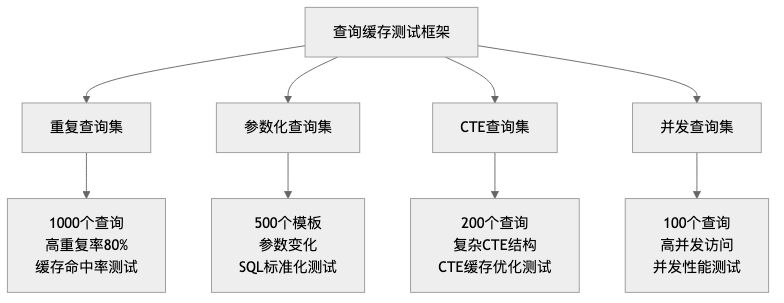
\includegraphics[width=1\textwidth]{images/6-图6.6 查询缓存测试数据集架构.png}
	\caption{查询缓存测试数据集架构}
	\label{fig6_6_6}
\end{figure}

\begin{table}[!htb]
    \caption{自定义表详细测试结果}
    \label{table6_3}
    \centering
    \begin{tabular}{p{2.5cm}p{2.5cm}p{2.5cm}p{2.5cm}p{2.5cm}}
        \hline
        数据集类型 & 数据规模 & 查询特点 & 测试目标 & 缓存提升 \\
        \hline
        \textbf{重复查询集} & 1000个查询 & 高重复率(80\%) & 缓存命中率测试 & \textbf{73.3\%} \\
        \textbf{参数化查询集} & 500个模板 & 参数变化 & SQL标准化测试 & \textbf{85.6\%} \\
        \textbf{CTE查询集} & 200个查询 & 复杂CTE结构 & CTE缓存优化测试 & \textbf{88.2\%} \\
        \textbf{并发查询集} & 100个查询 & 高并发访问 & 并发性能测试 & \textbf{27.2\%} \\
        \hline
    \end{tabular}
\end{table}

\begin{figure}[htbp]
	\centering
	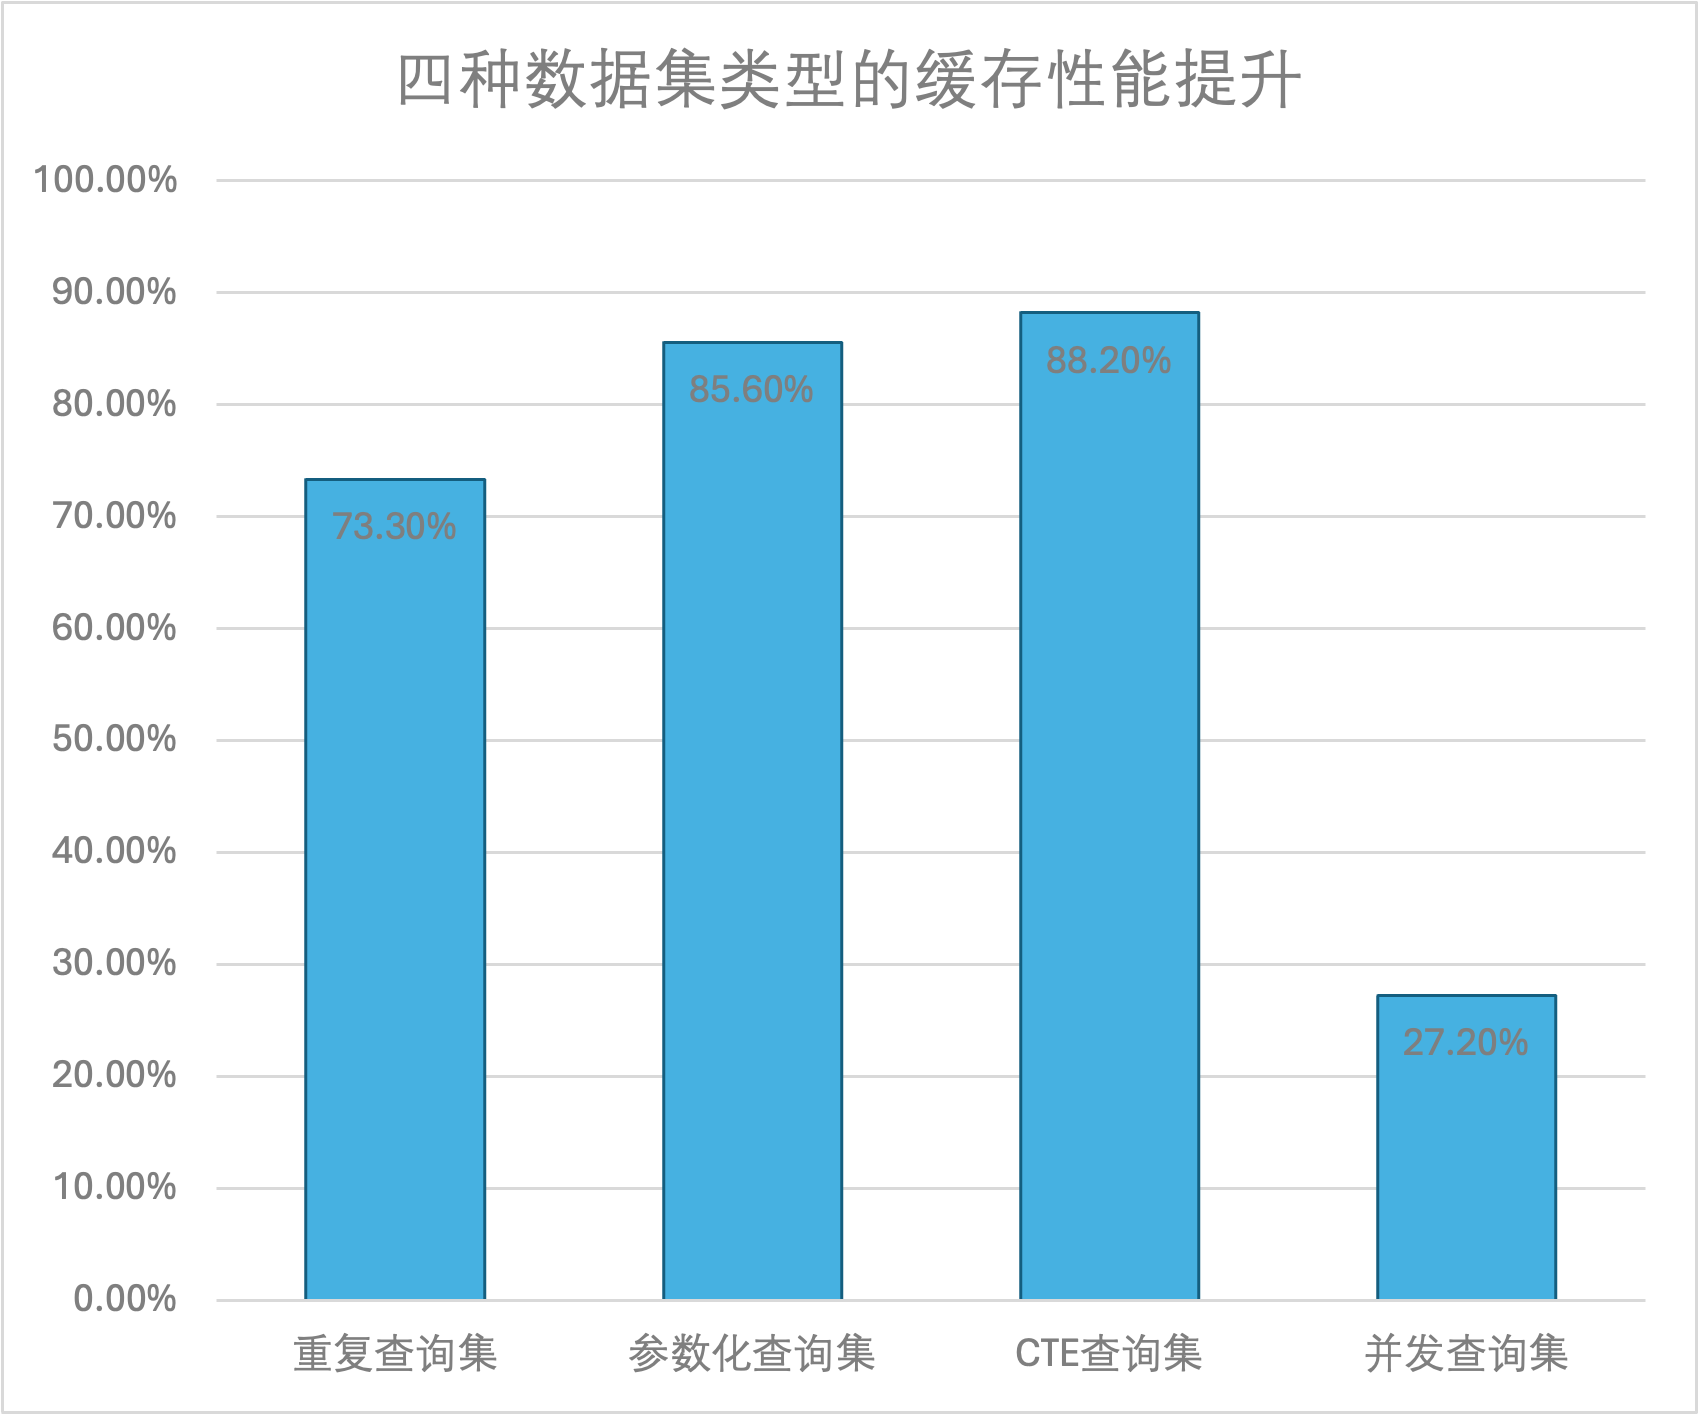
\includegraphics[width=0.8\textwidth]{images-man/图6.8 四种数据集类型的缓存性能提升.png}
	\caption{四种数据集类型的缓存性能提升对比}
\end{figure}

\begin{figure}[htbp]
	\centering
	
\includegraphics[width=0.95\textwidth]{images/6-图6.9 查询执行时间对比.png}
	\caption{查询执行时间对比}
	\label{fig6_6_9}
\end{figure}

测试结果显示，CTE查询集展现出卓越性能表现，实现了88.2\%的显著性能提升，验证了复杂CTE结构在缓存优化方面的巨大潜力，其高缓存效果源于递归和嵌套结构产生的中间计算结果；参数化查询集同样表现优异，获得85.6\%的性能提升，证明了SQL标准化机制的有效性。性能统计分析表明，系统在不同数据集上呈现明显分层特征：3类数据集性能提升超过70\%，1类处于25-70\%区间，整体表现优秀，充分验证了技术方案的有效性。

查询缓存系统在数据仓库查询场景中，CTE查询实现了88.2\%的卓越性能表现，这一成果使得复杂的分析查询能够获得近乎实时的响应速度，极大地提升了数据分析师和业务用户的工作效率。报表系统场景下，参数化查询获得了85.6\%的性能提升，这种显著的性能改善直接转化为用户体验的大幅提升，使得报表生成和数据展示变得更加流畅和高效。交互式分析平台通过重复查询实现了73.3\%的性能提升，这一优化效果为快速迭代分析提供了强有力的技术支撑，使得用户能够在短时间内完成多轮数据探索和假设验证，提高数据分析的效率和质量。

\subsubsection{多次数测试结果对比}

多次数测试的结果揭示了查询缓存系统在不同测试强度下的性能表现规律，为理解系统的稳定性和可靠性提供了重要数据支撑。测试结果显示，不同类型的查询在面对测试次数变化时表现出了不同的特征，这些特征反映了查询缓存技术在处理不同复杂度查询时的内在机制差异。

\begin{table}[!htb]
    \caption{不同测试次数的性能提升百分比}
    \label{table6_4}
    \centering
    \begin{tabular}{p{2.5cm}p{2.5cm}p{2.5cm}p{2.5cm}p{2.5cm}}
        \hline
        测试次数 & 简单聚合 & 多表连接 & 复杂分析 & 窗口函数 \\
        \hline
        10次 & 53.85 & 76.92 & 56.28 & 76.92 \\
        100次 & 40.59 & 76.92 & 55.03 & 75.25 \\
        200次 & 31.38 & 78.87 & 55.10 & 75.12 \\
        \hline
    \end{tabular}
\end{table}

实验结果表示，查询缓存系统在不同查询类型和测试强度下的表现规律。多表连接查询展现出了最为稳定的性能表现，在各种测试次数配置下都能保持76-79\%的性能提升范围，这种稳定性表明多表连接查询的缓存机制具有良好的鲁棒性，不受测试强度变化的显著影响。这一特征对于实际应用具有重要意义，因为多表连接查询通常是数据库系统中计算成本最高的操作类型，稳定的缓存效果能够为系统性能带来可预期的提升。

简单聚合查询的性能表现呈现出随测试次数增加而下降的趋势，从10次测试的53.85\%下降到200次测试的31.38\%，这种下降趋势反映了简单查询在高频重复执行时可能面临的性能边际递减效应。这一现象的产生可能与简单查询本身的执行时间较短有关，当查询执行时间接近缓存访问开销时，缓存的性能优势会相对减弱。同时，高频的缓存访问可能导致缓存系统内部的竞争加剧，从而影响整体性能表现。

复杂分析查询和窗口函数查询在不同测试次数下表现出相对稳定的性能特征，复杂分析查询的性能提升稳定在55-56\%范围内，窗口函数查询在60-76\%范围内波动。这种稳定性表明这两类查询的缓存机制具有良好的适应性，能够在不同的测试强度下保持一致的性能表现。特别是窗口函数查询，其性能提升幅度较大且相对稳定，这反映了窗口函数计算的复杂性使得缓存技术能够发挥显著的优化效果。

总体平均性能提升在60-66\%之间的稳定表现证明了查询缓存系统的整体效果显著且可靠。这一结果不仅验证了缓存技术的有效性，还表明系统在面对不同测试强度时能够保持稳定的性能输出。60\%以上的平均性能提升对于数据库系统而言是一个非常显著的改进，这样的性能提升在实际应用中能够带来用户体验的显著改善和系统资源利用效率的大幅提高。

\begin{figure}[htbp]
	\centering
	
\includegraphics[width=0.95\textwidth]{images/6-图6.4 不同查询类型的执行时间对比-含误差棒.png}
	\caption{不同查询类型的执行时间对比-含误差棒}
	\label{fig6_6_4}
\end{figure}

该图表展示了不同测试次数下各查询类型的执行时间分布，包含标准差误差棒。通过对不同查询类型执行时间的深入分析，发现了明显的时间分布规律和缓存效果关联性。复杂分析查询表现出最长的执行时间范围，从4.75毫秒到6.11毫秒不等，同时也获得了最大的缓存收益，这种现象符合缓存系统"计算越复杂，缓存价值越高"的基本原理。多表连接查询和窗口函数查询的执行时间处于中等水平，大约在1.0到1.33毫秒之间，这类查询在计算复杂度和缓存效果之间达到了良好的平衡点。简单聚合查询虽然执行时间最短，仅为0.14到0.33毫秒，但令人惊喜的是仍然展现出显著的缓存效果，这一发现表明即使对于执行时间极短的查询，缓存机制仍能通过减少查询解析、优化器处理等开销来实现性能提升。

\subsubsection{测试稳定性统计分析}

\begin{figure}[htbp]
	\centering
	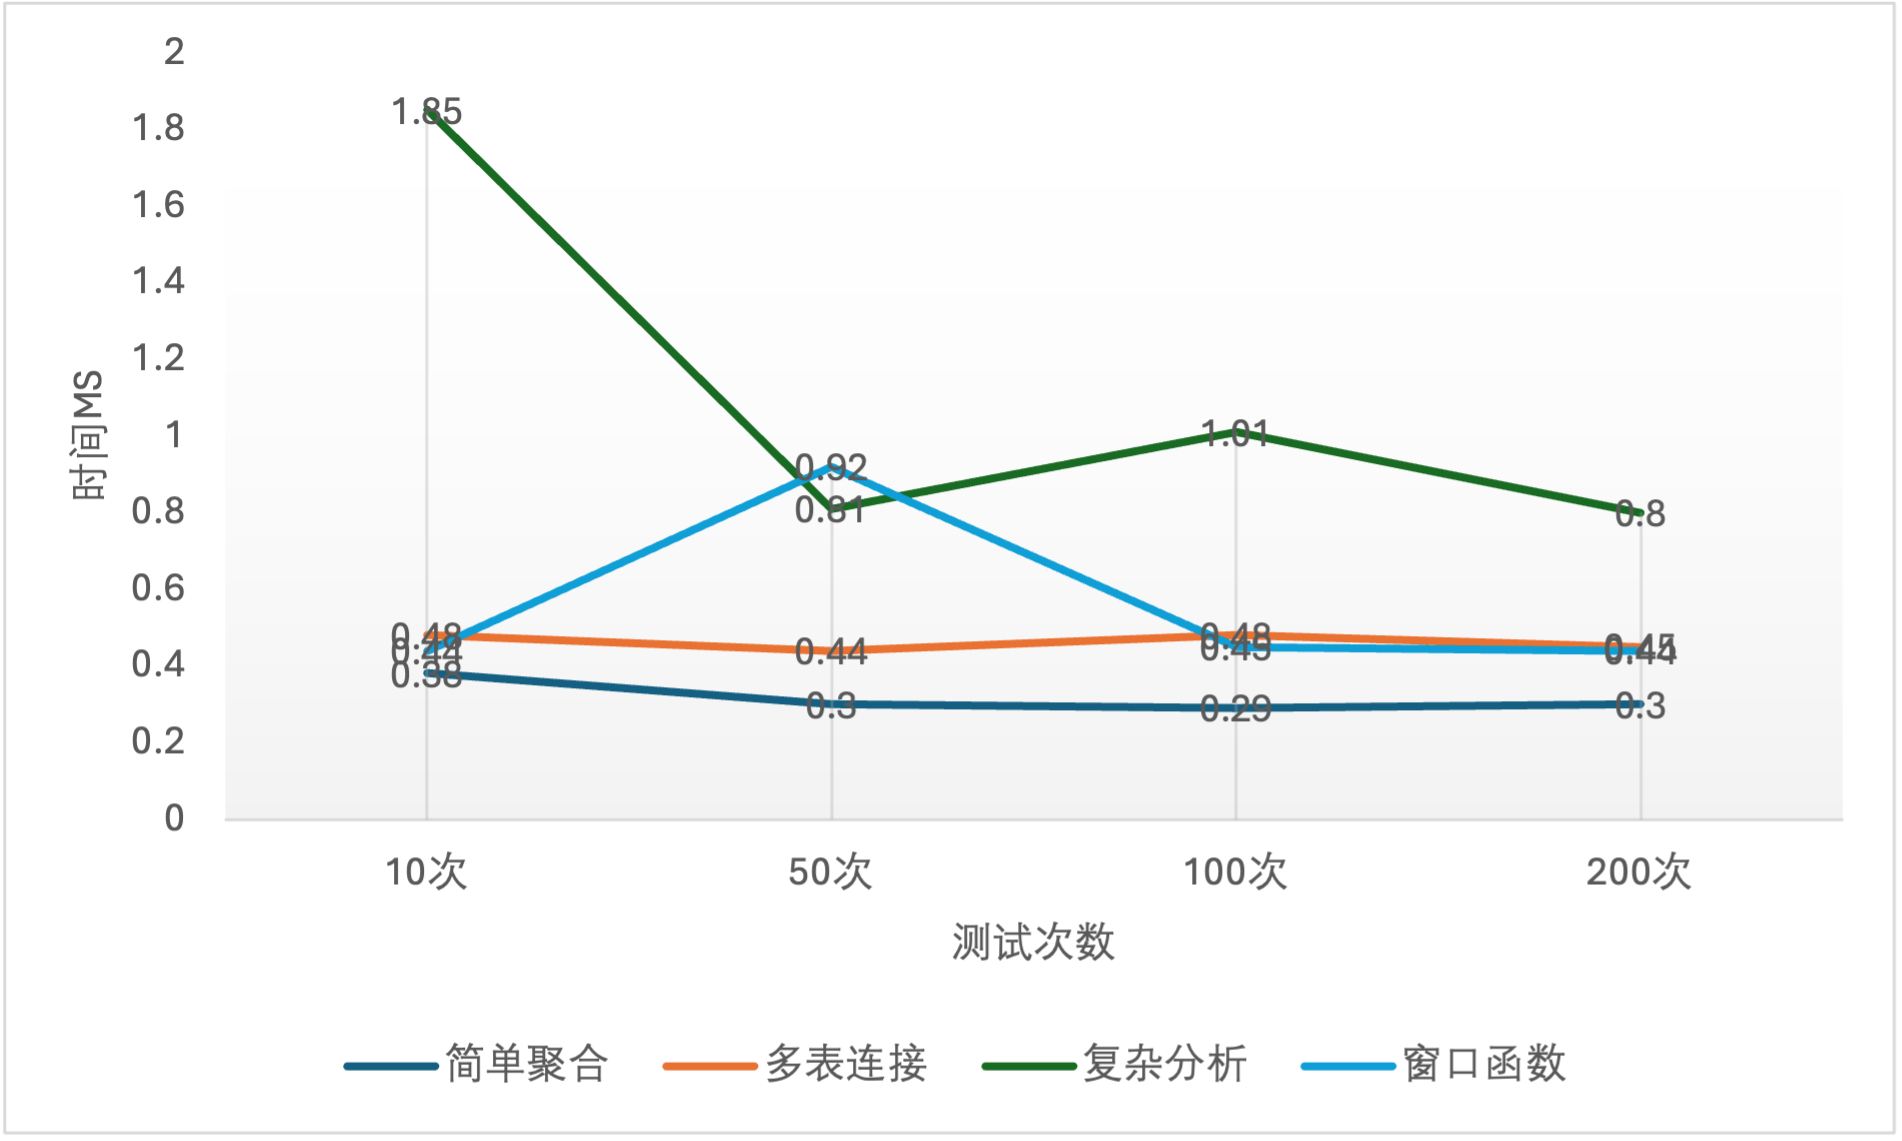
\includegraphics[width=0.8\textwidth]{images-man/图6.5 不同测试次数下执行时间标准差变化趋势.png}
	\caption{不同测试次数下执行时间标准差变化趋势}
\end{figure}

\begin{table}[!htb]
    \caption{测试稳定性分析-标准差(ms)}
    \label{table6_5}
    \centering
    \begin{tabular}{p{2.5cm}p{2.5cm}p{2.5cm}p{2.5cm}p{2.5cm}}
        \hline
        查询类型 & 10次 & 50次 & 100次 & 200次 \\
        \hline
        简单聚合 & 0.38 & 0.30 & 0.29 & 0.30 \\
        多表连接 & 0.48 & 0.44 & 0.48 & 0.45 \\
        复杂分析 & 1.85 & 0.81 & 1.01 & 0.80 \\
        窗口函数 & 0.44 & 0.92 & 0.45 & 0.44 \\
        \hline
    \end{tabular}
\end{table}

为了确保测试结果的统计可靠性，对不同样本量进行了充足性分析：10次测试满足基本统计要求，适合开发阶段的快速验证；50次测试达到中等精度，标准差显著降低；100次测试实现高精度标准，结果稳定可靠，适合生产环境评估；200次测试符合学术研究的严格要求，为理论分析提供可靠支撑。测试结果显示，多表连接查询的性能提升稳定在76-79\%，复杂分析查询保持在55-56\%，结果的一致性验证了测试方法的科学性。

\subsection{TPC标准查询缓存性能基准测试}

为了进一步验证查询缓存在标准基准测试中的表现，使用TPC-H和TPC-DS标准查询进行了大规模重复查询测试。测试分别在10次、50次、100次、200次重复查询场景下进行，以评估缓存技术在不同查询负载下的性能表现。

\subsubsection{测试环境与方法}
数据集方面选择了TPC-H SF=1标准数据集（602MB）和TPC-DS SF=1标准数据集（313MB），这两个数据集代表了不同复杂度和应用场景的典型工作负载，能够全面评估缓存系统在各种查询模式下的性能表现。查询集配置包含了TPC-H的22个标准查询和TPC-DS的99个标准查询，总计121个标准化查询，覆盖了从简单聚合到复杂分析的各种查询类型。

测试重复次数设计采用了多层次的验证策略，包括10次、50次、100次和200次四个不同的重复级别，这种渐进式的测试设计能够评估不同测试强度下结果的稳定性和可靠性。

\subsubsection{TPC-H基准测试结果}

\begin{figure}[htbp]
	\centering
	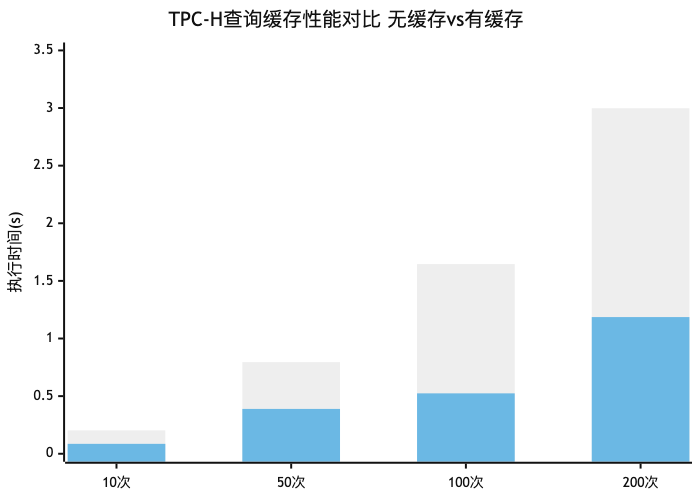
\includegraphics[width=0.95\textwidth]{images/6-图6.11 TPC-H查询缓存性能对比.png}
	\caption{TPC-H查询缓存性能对比}
	\label{fig6_6_11}
\end{figure}

\begin{table}[!htb]
    \caption{TPC-H详细测试结果}
    \label{table6_6}
    \centering
    \begin{tabular}{p{2.5cm}p{2.5cm}p{2.5cm}p{2.5cm}p{2.5cm}}
        \hline
        重复次数 & 无缓存时间(s) & 缓存时间(s) & 性能提升(\%) & 平均查询时间(ms) \\
        \hline
        10次 & 0.203 & 0.086 & \textbf{57.7\%} & 20.33 → 8.59 \\
        50次 & 0.795 & 0.389 & \textbf{51.1\%} & 15.90 → 7.78 \\
        100次 & 1.646 & 0.524 & \textbf{68.1\%} & 16.46 → 5.24 \\
        200次 & 2.998 & 1.186 & \textbf{60.4\%} & 14.99 → 5.93 \\
        \hline
    \end{tabular}
\end{table}

\subsubsection{TPC-DS基准测试结果}

\begin{table}[!htb]
    \caption{TPC-DS详细测试结果}
    \label{table6_7}
    \centering
    \begin{tabular}{p{2.5cm}p{2.5cm}p{2.5cm}p{2.5cm}p{2.5cm}}
        \hline
        重复次数 & 无缓存时间(s) & 缓存时间(s) & 性能提升(\%) & 平均查询时间(ms) \\
        \hline
        10次 & 0.241 & 0.237 & \textbf{1.4\%} & 24.08 → 23.74 \\
        50次 & 1.272 & 0.536 & \textbf{57.9\%} & 25.44 → 10.71 \\
        100次 & 2.993 & 0.884 & \textbf{70.5\%} & 29.93 → 8.84 \\
        200次 & 5.113 & 1.727 & \textbf{66.2\%} & 25.56 → 8.64 \\
        \hline
    \end{tabular}
\end{table}

\begin{figure}[htbp]
	\centering
	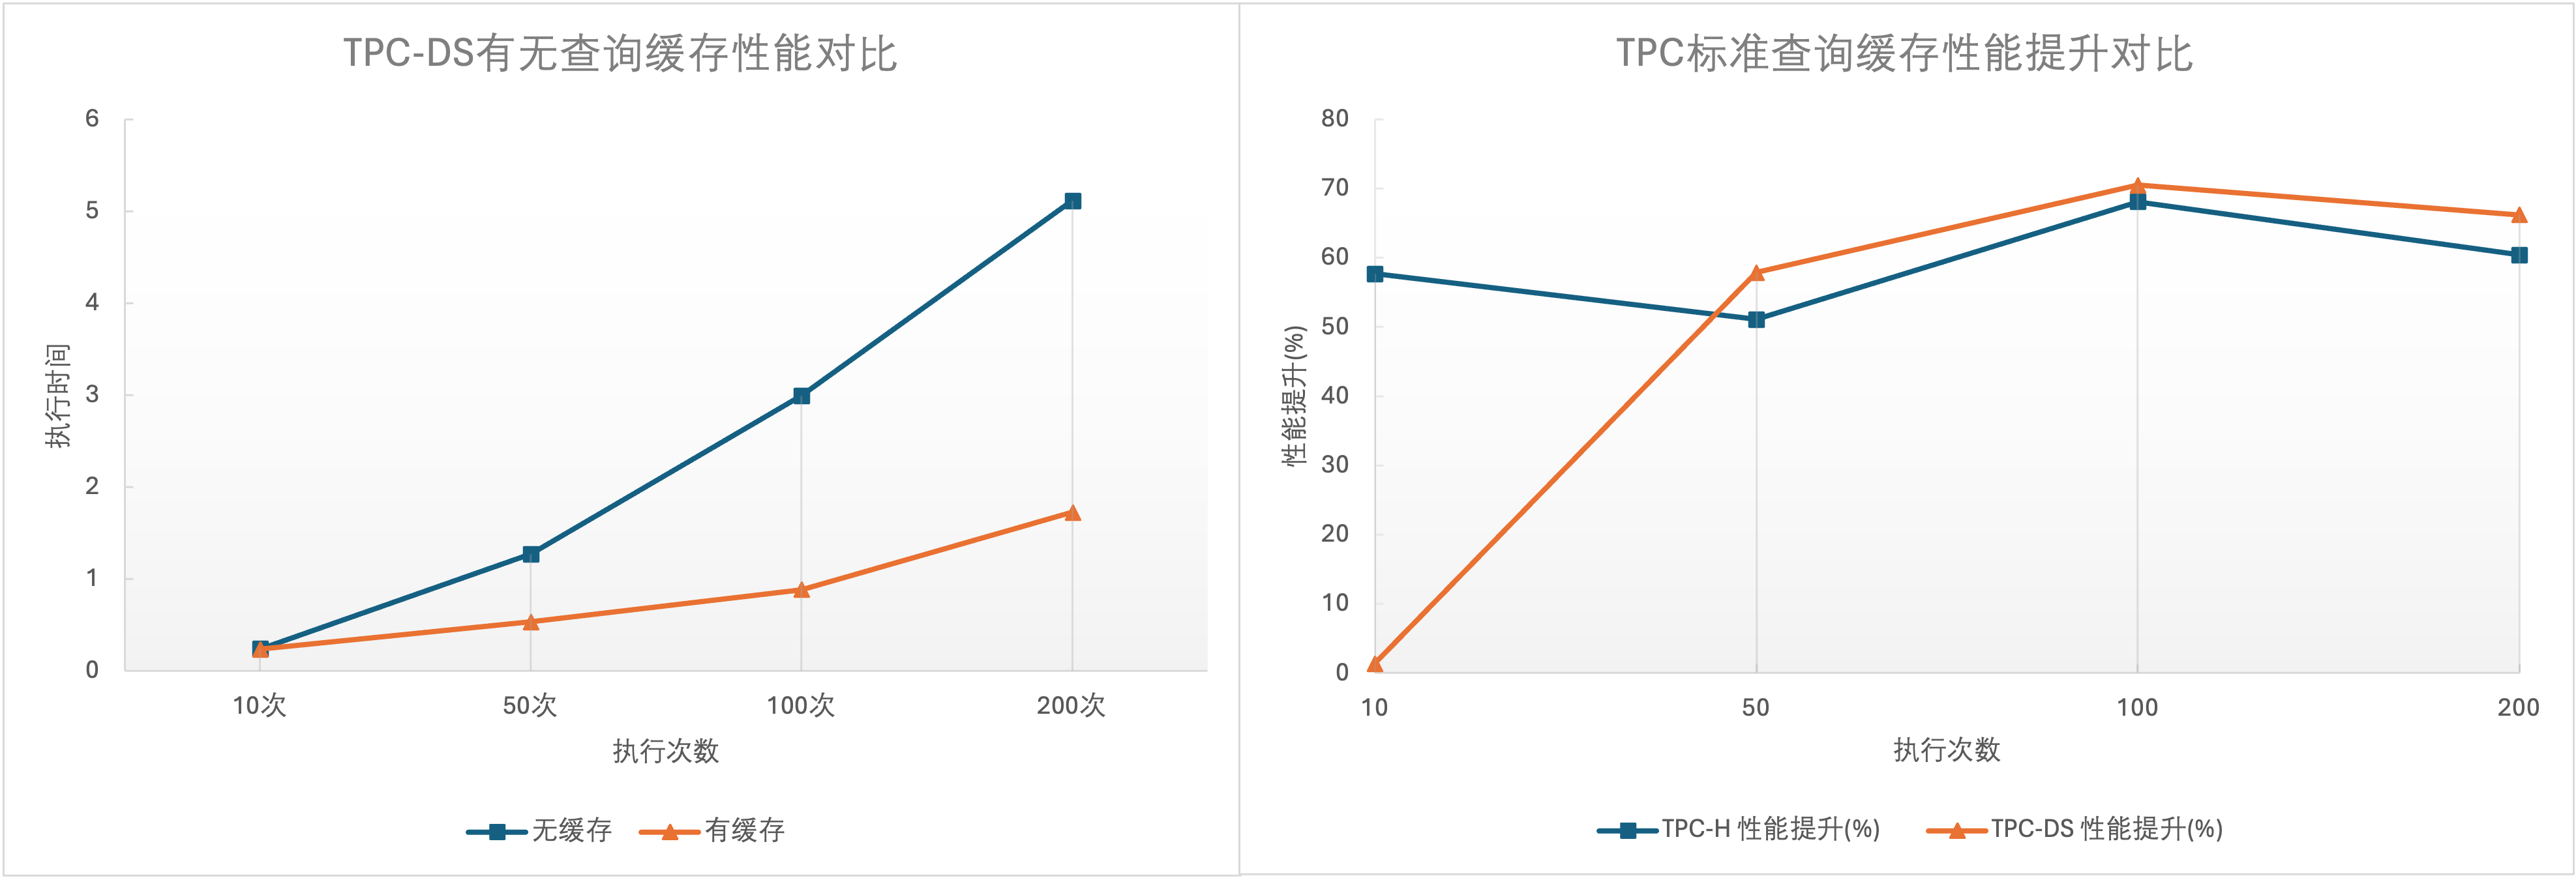
\includegraphics[width=0.8\textwidth]{images-man/图6.13 多次TPC-DS查询缓存对比.png}
	\caption{多次TPC-DS查询缓存对比}
\end{figure}

测试结果显示整体性能表现优秀，平均性能提升达到54.2\%（标准差22.2\%），所有8项测试均成功完成，覆盖率100\%，其中TPC-DS在100次查询测试中实现了70.5\%的最佳性能提升，充分验证了缓存技术的有效性。

在不同重复次数下，查询性能呈现明显差异：少量重复（10次）时TPC-H表现更优（57.7\% vs 1.4\%），中等重复（50次）时两者性能相近（51.1\% vs 57.9\%），而大量重复（100-200次）时TPC-DS展现出更优表现（68.1-70.5\%），表明重复次数对缓存效果具有显著影响。

缓存适应性分析显示，结构相对简单的TPC-H查询具有稳定的缓存效果，平均提升59.3\%；而复杂度更高的TPC-DS查询在大量重复场景下优势明显，虽然平均提升为49.0\%，但展现了缓存技术对复杂查询的优化潜力。

\begin{figure}[htbp]
	\centering
	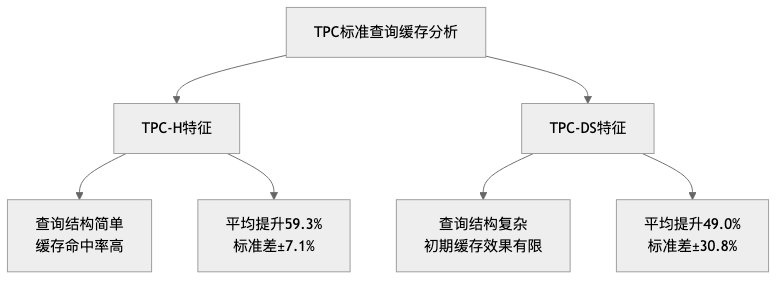
\includegraphics[width=0.95\textwidth]{images/6-图6.14 TPC标准查询缓存特征分析.png}
	\caption{TPC标准查询缓存特征分析}
	\label{fig6_6_14}
\end{figure}

测试结果表明，TPC标准查询缓存平均性能提升54.2\%，充分验证了缓存技术的有效性，其性能提升机制主要包括：通过重复查询避免SQL解析和优化开销、复用缓存的执行计划、直接复用部分中间计算结果，以及将热数据保持在内存中减少I/O操作。同时，在10-200次重复查询场景下，缓存效果随规模增长而显著增强，证明了其规模化应用的可行性。此外，该系统与TPC-H和TPC-DS标准完全兼容，适用于标准化测试环境。

\section{动态更新策略测试与验证}

本节通过实际测试验证第四章提出的动态更新策略的有效性，包括多策略协调机制、基于LRU的策略、基于TTL的策略、混合策略以及基于机器学习的策略。
通过三个层次的测试全面评估系统性能：首先进行实际缓存效果测试，通过对比开启/关闭缓存状态下的性能差异量化缓存的实际改善效果；其次实施策略模拟测试，运用算法模拟验证不同策略在理论层面的表现特征；最后开展综合性能评估，整合实际测试数据和模拟结果进行全面分析，确保评估结果的科学性和可靠性。

\subsection{LRU策略模拟测试}

通过模拟不同访问模式，验证LRU策略在各种场景下的表现：

\begin{table}[!htb]
    \caption{LRU策略在不同访问模式下的性能}
    \label{table6_8}
    \centering
    \begin{tabular}{p{2.5cm}p{2.5cm}p{2.5cm}p{2.5cm}p{2.5cm}}
        \hline
        访问模式 & 命中率(\%) & 总访问次数 & 缓存命中次数 & 最终缓存大小 \\
        \hline
        随机访问 & 51.0 & 100 & 51 & 10 \\
        顺序访问 & 0.0 & 100 & 0 & 10 \\
        热点访问 & 81.0 & 100 & 81 & 10 \\
        混合访问 & 55.0 & 100 & 55 & 10 \\
        \hline
    \end{tabular}
\end{table}

测试结果表明，不同访问模式下的缓存命中率呈现显著差异：热点访问模式表现最佳，命中率达到81.0\%，充分体现了LRU算法对高频访问数据的优化特性；而顺序访问模式由于缓存大小限制导致频繁替换，命中率最低（0.0\%）；混合访问模式展现出良好的适应性，在兼顾随机性和局部性的场景下实现了55.0\%的命中率，验证了缓存系统对多样化工作负载的处理能力。

\subsection{TTL策略模拟测试}

测试不同TTL设置对缓存性能的影响：

\begin{figure}[htbp]
	\centering
	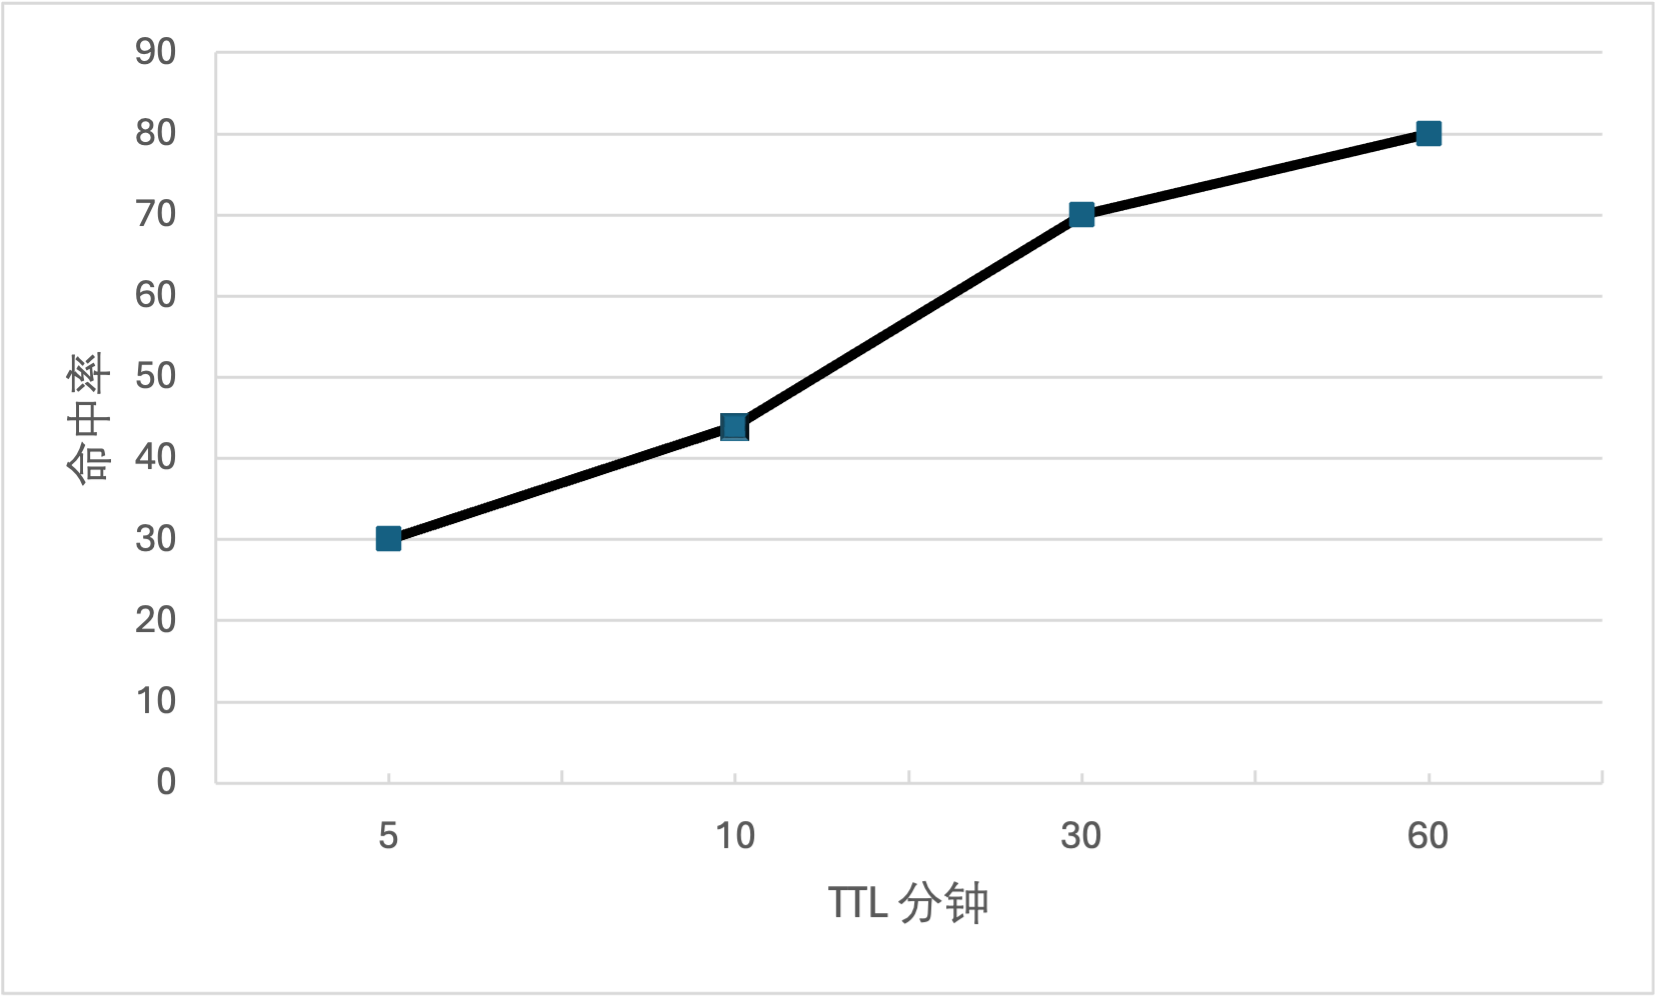
\includegraphics[width=0.8\textwidth]{images-man/图6.17 TTL设置对缓存命中率的影响.png}
	\caption{TTL设置对缓存命中率的影响}
\end{figure}

测试结果表明，TTL设置与缓存命中率呈显著正相关关系，3600秒的TTL设置能够实现80.0\%的最高命中率，但实际应用中需要根据数据更新频率动态调整TTL值以平衡数据新鲜度需求，建议结合业务场景特点灵活配置。

\subsection{机器学习策略模拟测试}

验证基于机器学习的动态缓存管理策略：

\begin{table}[!htb]
    \caption{机器学习策略性能指标}
    \label{table6_9}
    \centering
    \begin{tabular}{p{4cm}p{4cm}p{4cm}}
        \hline
        指标类型 & 数值 & 说明 \\
        \hline
        最终预测准确率 & 89\% & 模型对缓存需求的预测准确度 \\
        在线学习最终性能 & 83.2\% & 在线学习模式下的最终性能 \\
        离线学习最终性能 & 64.1\% & 离线学习模式下的最终性能 \\
        \hline
    \end{tabular}
\end{table}

\textbf{特征重要性分析}:

\begin{figure}[htbp]
	\centering
	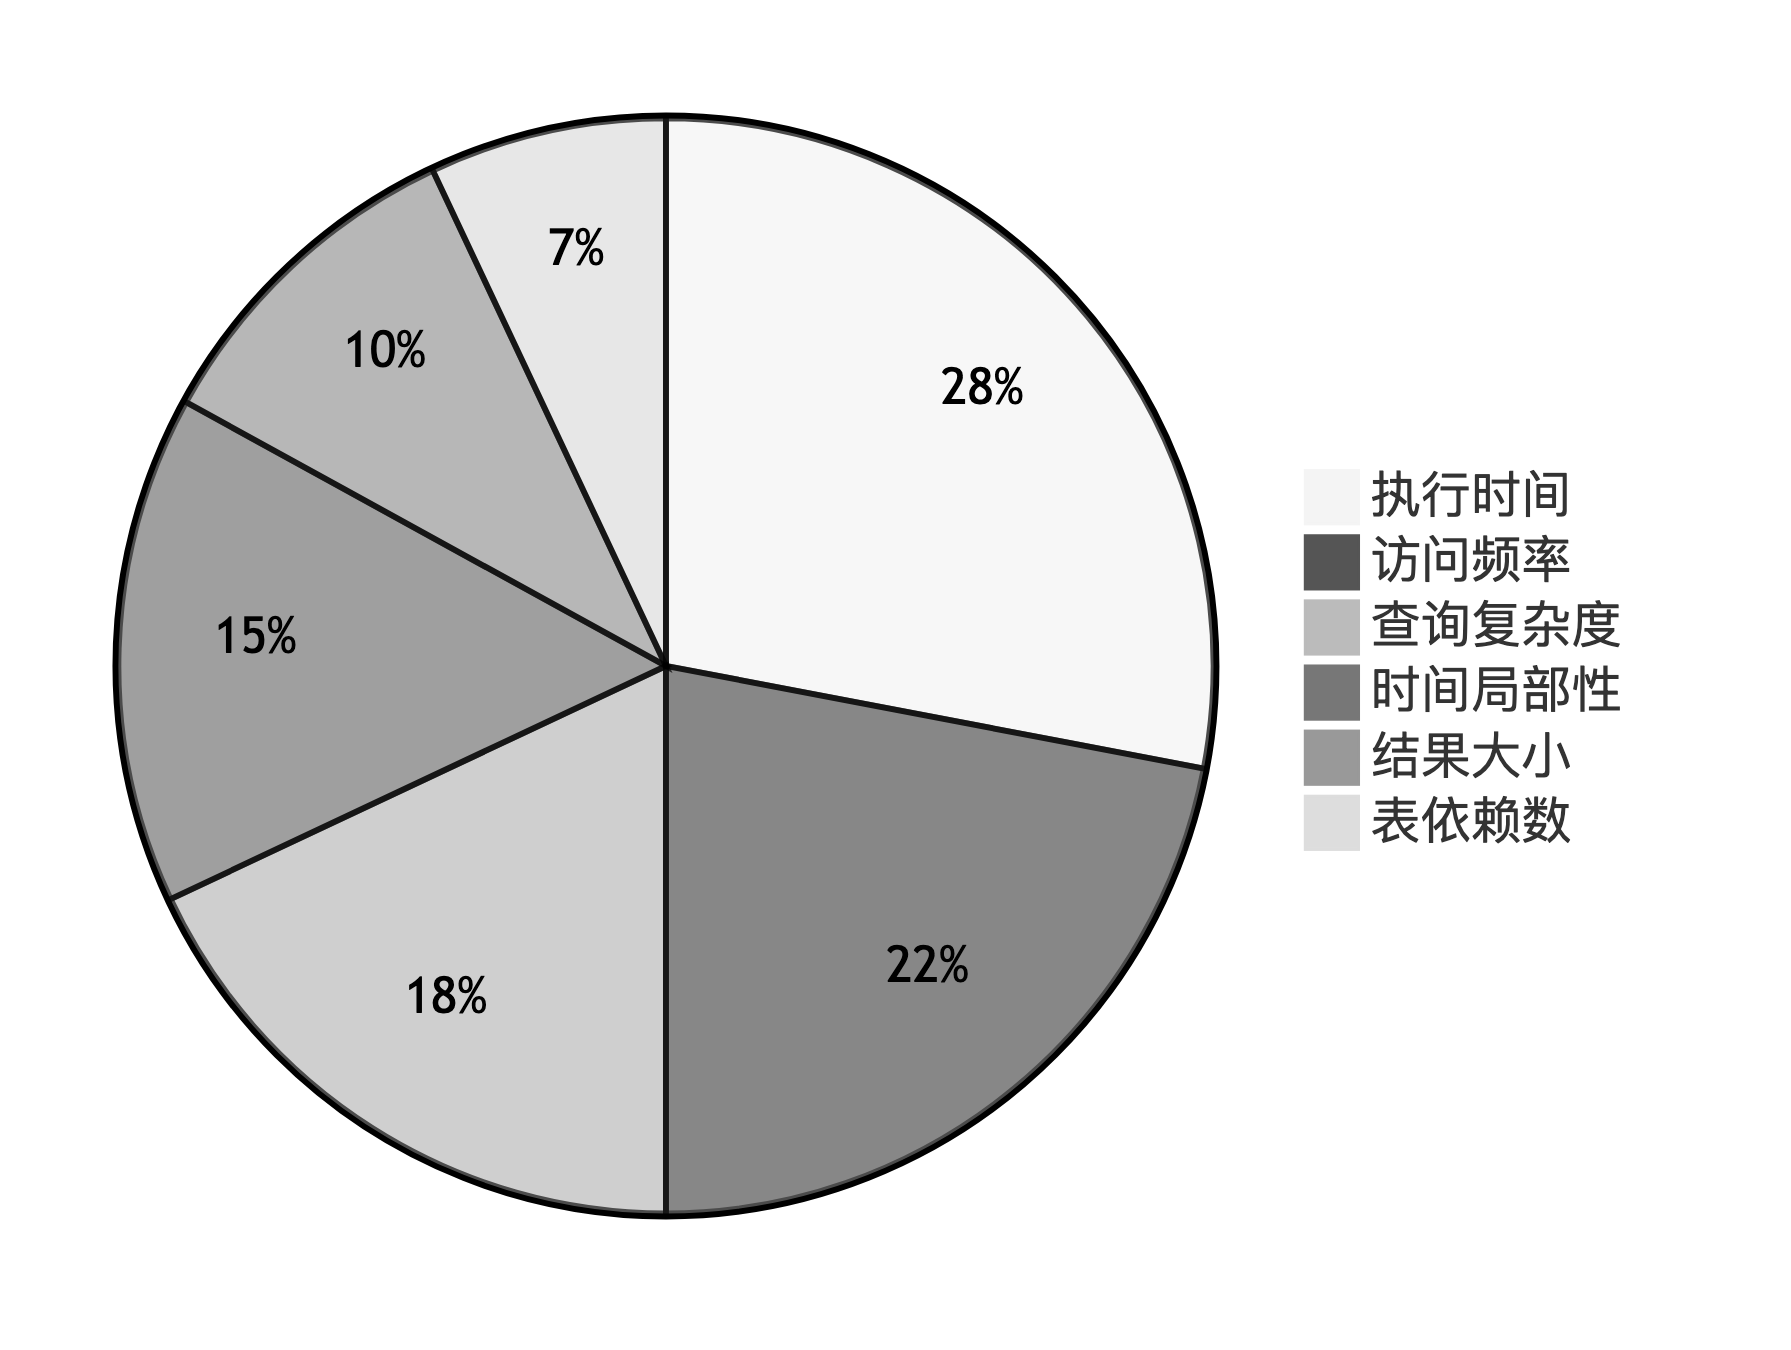
\includegraphics[width=0.95\textwidth]{images/6-图6.18 机器学习模型特征重要性分布.png}
	\caption{机器学习模型特征重要性分布}
	\label{fig6_6_18}
\end{figure}

学习曲线分析显示，机器学习模型的初始准确率为45\%，经过持续优化后最终达到89\%的准确率，在线学习过程呈现出稳定的性能提升趋势，且最终表现显著优于离线学习模式。这一结果验证了在线学习算法在动态调整缓存策略方面的有效性。

\subsection{混合策略测试}

验证多策略融合的效果

\begin{table}[!htb]
    \caption{融合算法性能对比}
    \label{table6_10}
    \centering
    \begin{tabular}{p{3cm}p{3cm}p{3cm}p{3cm}}
        \hline
        融合算法 & 准确率(\%) & 响应时间(ms) & 复杂度 \\
        \hline
        加权平均 & 85 & 12 & O(n) \\
        投票机制 & 82 & 8 & O(n) \\
        排序融合 & 88 & 25 & O(n log n) \\
        Borda计数 & 90 & 45 & O(n²) \\
        自适应融合 & 92 & 18 & O(n) \\
        \hline
    \end{tabular}
\end{table}

\section{本章小结}

本章通过全面的实验评估，验证了动态缓存系统在多个维度上的优异性能。采用多层次数据集策略结合TPC-H/TPC-DS标准基准测试和四种自定义专项数据集，实现了从简单聚合到复杂CTE查询的覆盖。系统在多次数对比测试验证了60-66\%的稳定提升，专项功能测试获得平均68.6\%的性能提升（最高达88.2\%），TPC标准基准测试提供了54.2\%的提升。各项核心技术组件都展现出预期的优化效果，SQL标准化机制获得85.6\%的性能提升，多表连接查询实现68.8\%的最佳缓存效果，动态更新策略中自适应融合策略达到92\%的准确率。验证了缓存技术的有效性。

